\documentclass[a4paper,12pt, openany,oneside]{book}
\usepackage{graphicx}
\usepackage{hyperref}
\pagestyle{plain}
\usepackage[italian]{babel}
\usepackage{picture}
\usepackage{hyperref}
\usepackage[Symbol]{upgreek}
\usepackage{amsmath}
\usepackage{listings}
\usepackage[utf8]{inputenc}
%\usepackage{showframe}
\usepackage{float}
\usepackage{algorithm, algpseudocode}
\usepackage{tikz}
\usetikzlibrary{shapes,arrows,shapes.multipart}
\usepackage{geometry,lipsum,graphicx}
\usepackage{pdfpages}
\usepackage{csquotes}
\usepackage{enumitem}
\usepackage{wrapfig}
\usepackage{biblatex}
\addbibresource{bibliography.bib}
\addbibresource{web.bib}
\usepackage{xcolor}
\usepackage{subcaption}
\usepackage{cleveref}

\lstdefinelanguage{docker}{
  basicstyle=\scriptsize \ttfamily \color{black} \bfseries,
  keywords={FROM, RUN, COPY, ADD, ENTRYPOINT, CMD,  ENV, ARG, WORKDIR, EXPOSE, LABEL, USER, VOLUME, STOPSIGNAL, ONBUILD, MAINTAINER},
  keywordstyle=\color{blue}\bfseries,
  identifierstyle=\color{black},
  sensitive=false,
  comment=[l]{\#},
  commentstyle=\color{purple}\ttfamily,
  stringstyle=\color{red}\ttfamily,
  morestring=[b]',
  morestring=[b]",
  showspaces=false,               
  showstringspaces=false,        
  showtabs=false,                
  stepnumber=1,                   
  tabsize=5,                     
  title=\lstname,
  frame=bt,
  numberstyle=\tiny\color{orange}, 
  rulecolor=\color{black},
  aboveskip=5mm,
  belowskip=-5mm, 
  breakatwhitespace=false,       
  breaklines=true            
}

\lstdefinelanguage{cpp}{
      %backgroundcolor=\color{lgrey},  
      basicstyle=\scriptsize \ttfamily \color{black} \bfseries,  
      aboveskip=5mm,
      belowskip=-5mm, 
      breakatwhitespace=false,       
      breaklines=true,               
      captionpos=b,                   
      commentstyle=\color{dkgreen},   
      deletekeywords={...},          
      escapeinside={\%*}{*)},                  
      frame=bt,                  
      language=C++,                
      keywordstyle=\color{purple},  
      morekeywords={BRIEFDescriptorConfig,string,TiXmlNode,DetectorDescriptorConfigContainer,istringstream,cerr,exit,pcl}, 
      identifierstyle=\color{black},
      stringstyle=\color{blue},   
      keywordstyle=\color{green},
      numbersep=5pt,                  
      numberstyle=\tiny\color{orange}, 
      rulecolor=\color{black},        
      showspaces=false,               
      showstringspaces=false,        
      showtabs=false,                
      stepnumber=1,                   
      tabsize=5,                     
      title=\lstname,   
    }
    
    \lstdefinelanguage{xml}{
      %backgroundcolor=\color{lgrey},  
      basicstyle=\scriptsize,
      aboveskip=5mm,
      belowskip=-5mm, 
      belowcaptionskip=0mm,  
      breakatwhitespace=false,       
      breaklines=true,               
      captionpos=b,                   
      commentstyle=\color{gray},            
      frame=bt,       
      morestring=[b]",
      morestring=[s]{>}{<},
      morecomment=[s]{<?}{?>},
      stringstyle=\color{black},
      identifierstyle=\color{darkblue},
      keywordstyle=\color{cyan},
      morekeywords={xmlns,version,type,ira_open_street_map}          
      %language=XML,      
      numbers=none,                 
      numbersep=5pt,                  
      numberstyle=\tiny\color{black},       
      showspaces=false,               
      showstringspaces=false,        
      showtabs=false,                
      stepnumber=1,                   
      tabsize=5,
      escapeinside={<@}{@>},                     
      title=\lstname,                 
    }
    
\iffalse
\lstset{ %
  %language=XML,                % the language of the code
  basicstyle=\tiny,           % the size of the fonts that are used for the code
  numbers=left,                   % where to put the line-numbers
  numberstyle=\tiny\color{gray},  % the style that is used for the line-numbers
  stepnumber=1,                   % the step between two line-numbers. If it's 1, each line  will be numbered
  numbersep=5pt,                  % how far the line-numbers are from the code
  backgroundcolor=\color{white},      % choose the background color. You must add \usepackage{color}
  showspaces=false,               % show spaces adding particular underscores
  showstringspaces=false,         % underline spaces within strings
  showtabs=false,                 % show tabs within strings adding particular underscores
  frame=none,                   % adds a frame around the code
  rulecolor=\color{black},        % if not set, the frame-color may be changed on line-breaks within not-black text (e.g. commens (green here))
  tabsize=1,                      % sets default tabsize to 2 spaces
  captionpos=b,                   % sets the caption-position to bottom
  breaklines=true,                % sets automatic line breaking
  breakatwhitespace=false,        % sets if automatic breaks should only happen at whitespace
%   title=\lstname,                   % show the filename of files included with \lstinputlisting;
                                  % also try caption instead of title
  %identifierstyle=\color{magenta},
  keywordstyle=\color{blue},          % keyword style
  commentstyle=\color{dkgreen},       % comment style
  stringstyle=\color{mauve},         % string literal style
  escapeinside={-*}{*-},            % if you want to add a comment within your code
  morekeywords={*,...}               % if you want to add more keywords to the set
}
\fi

% Per Intestazione 
\usepackage{fancyhdr}
\pagestyle{fancy}
\fancyhf{}
\fancyhead[LE,RO]{\nouppercase{\leftmark}}
\fancyhead[RE,LO]{\thepage}

\begin{document} 
\begin{titlepage}
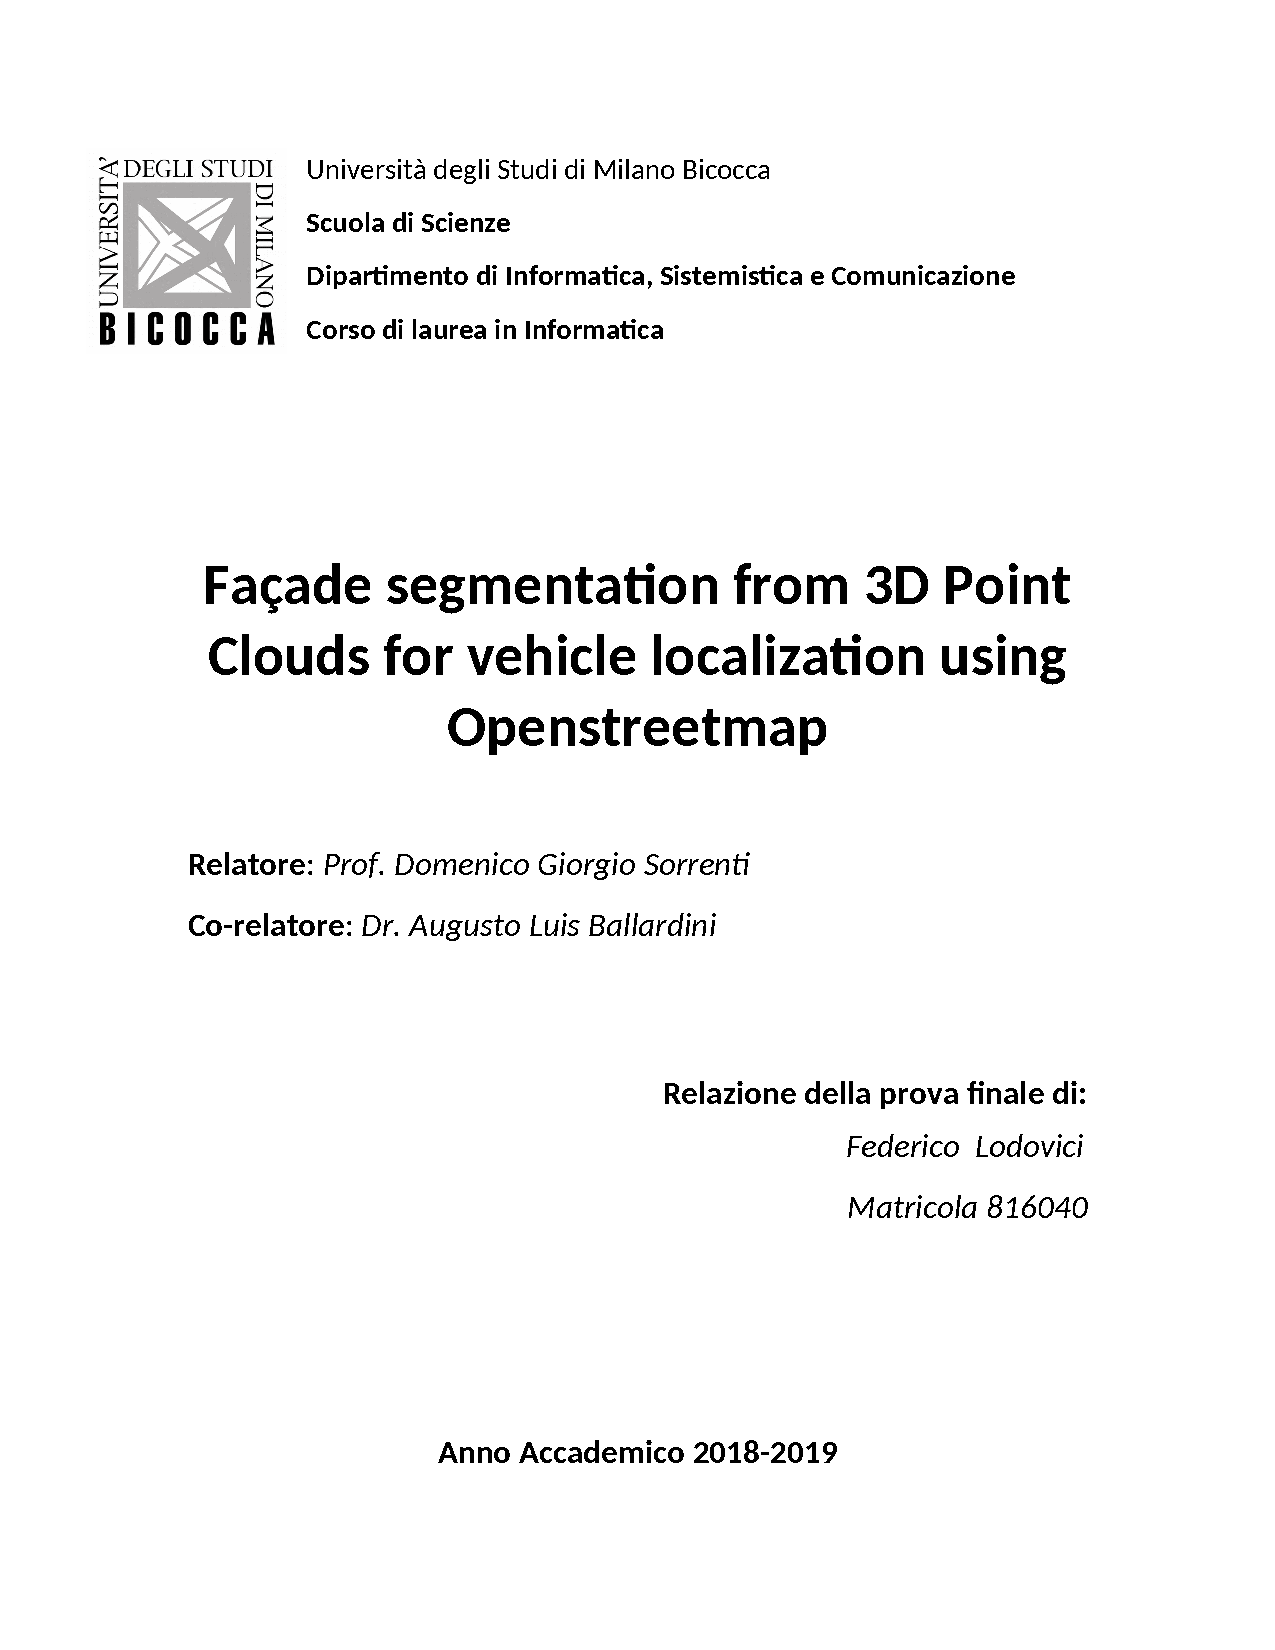
\includepdf[]{Immagini/L-I_Frontespizio-relazione-finale.pdf}
\end{titlepage}
\begin{flushright}
	\textit{    
	Basta seguire la strada \\
	e prima o poi si fa il giro del mondo. \\
	Non può finire in nessun altro posto, no? \\
	Jack Kerouac, On the Road
		}
\end{flushright}
\thispagestyle{empty}
\newpage
\tableofcontents
\newpage
\input{Capitoli/chap0.tex}
\input{Capitoli/chap1.tex}
\chapter{Inserimento in OpenStreetMaps}
\label{cap:PCLeOSM}
In questo capitolo si descriverà come sono state inserite le point cloud all'interno delle mappe e di come queste sono state messe a disposizione per l'utilizzo.

\section{OpenStreetMap}
\label{sez:OSM}

\begin{wrapfigure}{r}{0.3\linewidth}
    \vspace{-20pt}
        \begin{center}
            
\includegraphics[width=0.2\textwidth]{Immagini/OSMLogo.png}
        \end{center}
    \vspace{-20pt}
    \caption{OSM Logo}
\label{fig:OSMLogo}
\end{wrapfigure}

OpenStreet Map\cite{OSM} è un'iniziativa per creare e fornire dati geografici a chiunque gestita dalla OpenStreetMap Foundation. Essa permette di contribuire, accedere ai dati e  ospitare una propria infrastruttura privata senza la necessità di appoggiarsi a infrastrutture chiuse e proprietarie.
OpenStreetMap è un database che utilizza un proprio formato di scambio dati basato su XML, tutti gli elementi che possono essere inseriti e che modellano la realtà sono di quattro tipologie: 
\begin{enumerate}
    \item punto (node): singolo punto. E' utilizzato per indicare oggetti puntuali.
    \begin{figure}[H]
    \centering
    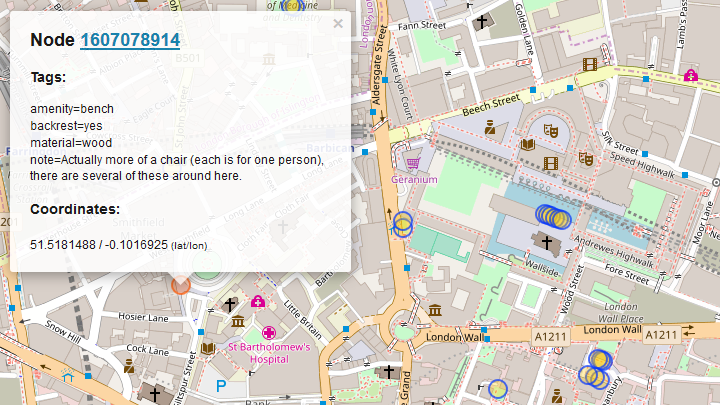
\includegraphics[width=0.5\textwidth]{Immagini/nodes.png}
    \caption{Node}
    \label{fig:OSMNode}
\end{figure}

    \item linea (way): un insieme di punti non chiuso, il percorso è un segmento tra punti che può descrivere oggetti che seguono una linea come vie, muri e simili.
    \begin{figure}[H]
    \centering
    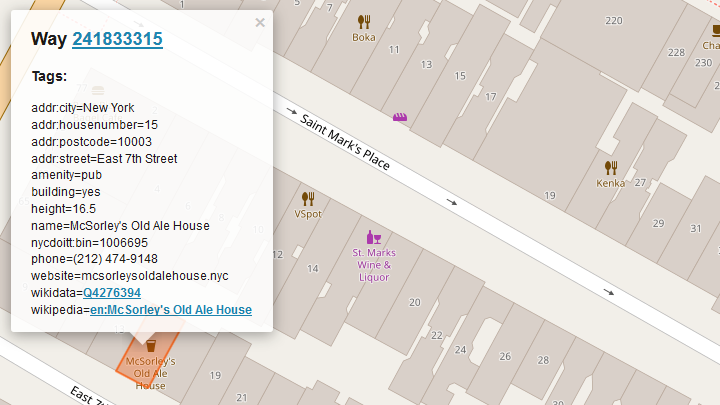
\includegraphics[width=0.5\textwidth]{Immagini/way.png}
    \caption{Way}
    \label{fig:OSMWay}
\end{figure}

    \item area (polygon): una linea chiusa ovvero un insieme di segmenti che si chiudono, è utilizzato per rappresentare oggetti che hanno un qualche tipo di area.
    \item relazione (relation): è un insieme degli elementi scritti sopra, esso consente di rappresentare oggetti complessi composti da un insieme di elementi.
    \begin{figure}[H]
    \centering
    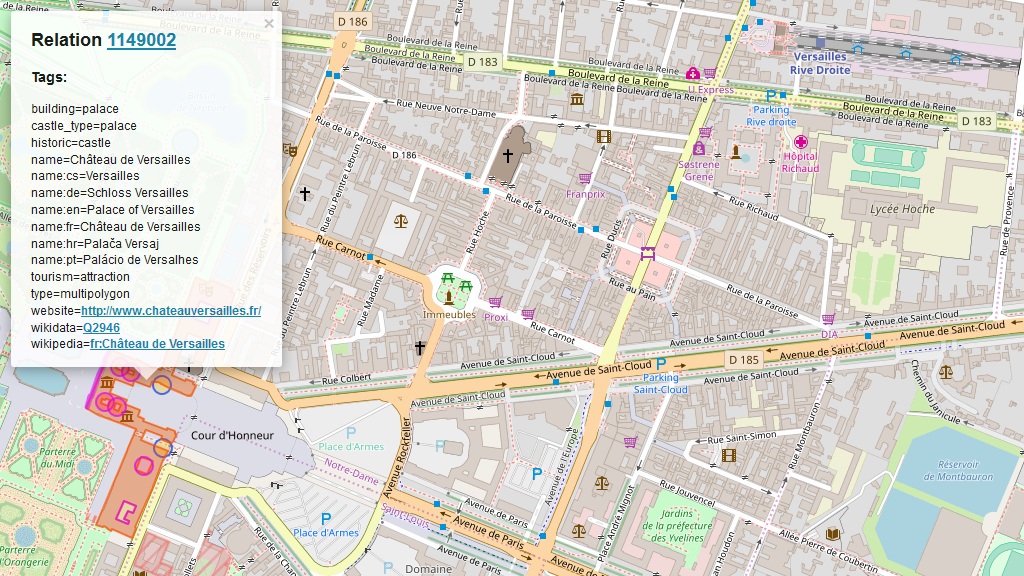
\includegraphics[width=0.5\textwidth]{Immagini/relation.png}
    \caption{Relation}
    \label{fig:OSMPolygon}
\end{figure}

\end{enumerate}{}
Nel progetto si sono manipolati elementi di tipo way e relation.
Per descrivere gli oggetti vengono utilizzate delle etichette (tag) che sono codificate secondo uno standard internazionale e sono composte da una tupla di elementi consistenti in una chiave (key) e un valore (value). Ogni oggetto dev'essere descritto da almeno un tag  principale per identificarlo ed è inoltre possibile aggiungerne di secondari che consentono di descrivere particolari proprietà. Il concetto di etichetta è stato utilizzato all'interno del progetto per consentire di aggiungere una chiave che possa descrivere la facciata di un edificio.

\section{JOSM}
\label{sez:JOSM}

\begin{wrapfigure}{r}{0.3\linewidth}
    \vspace{-20pt}
        \begin{center}
            
\includegraphics[width=0.2\textwidth]{Immagini/logoJOSM.png}
        \end{center}
    \vspace{-20pt}
    \caption{JOSM Logo}
\label{fig:JOSMLogo}
\end{wrapfigure}

JOSM\cite{josm} è un editor per OpenStreetMap(OSM) Open Source licenziato sotto GPL estensibile scritto in Java. Supporta l'editing avanzato delle mappe senza le limitazioni date dall'interfaccia web di OSM.
Consente inoltre il caricamento di tracciati GPX, l'utilizzo di immagini di backround, la modifica dei dati di OSM da sorgenti locali oltre che da sorgenti online. Consente inoltre di modificare tutte le tipologie di dato associate ad OSM e i loro tag.\newline
JOSM è stato scelto per la capacità di modificare in modo avanzato le mappe in particolare per poter modificare un'istanza locale di OSM e non dover modificare le mappe globali. 

\section{Docker}
\label{sez:Docker}

\begin{wrapfigure}{r}{0.3\linewidth}
    \vspace{-20pt}
        \begin{center}
            
\includegraphics[width=0.2\textwidth]{Immagini/LogoDocker.png}
        \end{center}
    \vspace{-20pt}
    \caption{Docker Logo}
\label{fig:DockerLogo}
\end{wrapfigure}

Docker\cite{docker} è un progetto open-source nato per automatizzare il deployment di applicazioni all'interno di contenitore che in Docker si chiama Container, fornendo un livello ulteriore di astrazione grazie alla virtualizzazione a livello di sistema operativo concesso da Linux.\newline

Docker utilizza le funzionalità di isolamento delle risorse del kernel Linux, come cgroup e namespace per consentire a container indipendenti di coesistere sulla stessa istanza di Linux, evitando l'installazione e la manutenzione di una macchina virtuale (VM): i namespace del kernel Linux isolano ciò che l'applicazione può vedere dell'ambiente operativo, incluso l'albero dei processi, la rete, gli ID utente e i file system montati, mentre i cgroup forniscono l'isolamento delle risorse, inclusa la CPU, la memoria, i dispositivi di I/O a blocchi e la rete.\newline

Docker accede alle funzionalità di virtualizzazione del kernel Linux o direttamente utilizzando la libreria libcontainer, che è disponibile da Docker 0.9, o indirettamente attraverso libvirt, LXC o systemd-nspawn. I container condividono lo stesso kernel, ma ciascuno di essi può dover utilizzare una certa quantità di risorse, come la CPU, la memoria e l'I/O.\newline

\section{Inserimento nelle mappe}
\label{sez:insmap}
Per associare i singoli cluster agli edifici si è deciso di intervenire andando ad aggiungere una nuova etichetta agli edifici che presentavano il tag building.\\
Il tag aggiunto è denominato \textit{building:facade:pcl}, ad esso viene associato come valore l'url presso cui è salvato l'oggetto pcd che contiene la facciata dell'edificio.\\
L'aggiunta del tag è stata fatta manualmente attraverso l'utilizzo di \hyperref[sez:JOSM]{JOSM}, come si può vedere nella figura successiva.

\begin{figure}[H]
    \centering
    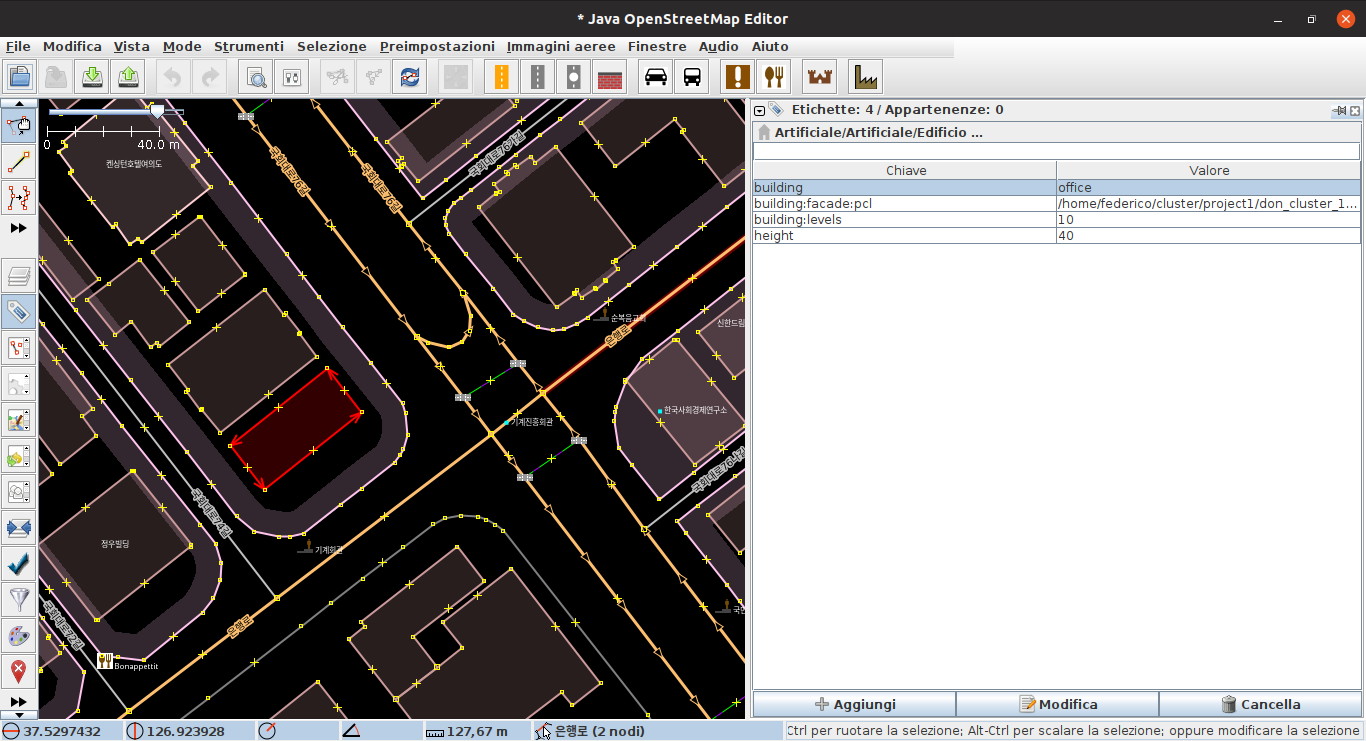
\includegraphics[width=0.9\textwidth]{Immagini/JOSMedit.png}
    \caption{Esempio di modifica di un edificio con JOSM}
    \label{fig:JOSMedit}
\end{figure}

Nel pannello di sinistra di può vedere il tracciato selezionato di tipo \textit{polygon} in quanto linea chiusa. 
Nel pannello di destra si possono invece evidenziare i tag associati allo specifico poligono, in particolare si può vedere che esso è un edificio e che vi è associato uno specifico cluster oltre che a dati di importanza secondaria come l'altezza dell'edifico o il numero di piani.
Il procedimento di associazione è stato ripetuto per ogni cluster precedentemente estratto, la mappa modificata è stata infine esportata per essere servita.

\subsection{Overpass API}
Per consentire l'estrazione delle informazioni si è deciso di utilizzare Overpass\cite{Overpass}.\\

Overpass API è un'API read-only che permette di servire i dati di regioni specifiche della mappa di OSM, funziona come un database, il client lancia una query all'API e riceve i dati che corrispondono alla query.\\

A differenza dell'API principale di OSM che è ottimizzata per l'editing, Overpass è ottimizzata per fornire pochi elementi in pochi secondi o fino a 10 milioni di elementi in pochi minuti entrambi filtrati da specifici criteri di ricerca. Funziona come backend per vari servizi.\\

Dal momento che non si voleva utilizzare la mappa globale ma una nostra versione modificata è stato necessario ospitare in locale un server Overpass, per poter far fronte alle difficoltà dovute all'utilizzo di versioni di librerie diverse e incompatibili tra loro si è deciso di utilizzare \hyperref[sez:Docker]{Docker} che permette di fare il deploy del server in un container portabile ed isolato.\\

Il container è stato costruito a partire da un container già esistente\cite{OverpassDocker} al quale sono state apportate modifiche per ottenere il seguente listato:
\begin{lstlisting}[caption={Dockerfile per OverpassAPI},captionpos=b,language=docker]

FROM ubuntu:16.04
RUN apt-get update 
RUN apt-get install -y apache2 vim
RUN apt-get install -y \
	autoconf \
	automake1.11 \
	expat \
	git \
	g++ \
	libtool \
	libexpat1-dev \
	make \
	zlib1g-dev \
	bzip2 \
	wget \
	liblz4-1 liblz4-dev
RUN apt-get clean && rm -rf /var/lib/apt/lists/*
RUN git clone https://github.com/drolbr/Overpass-API.git
WORKDIR /Overpass-API
#Checkout latest version
RUN git checkout $(git describe --abbrev=0 --tags)
#Configure
WORKDIR /Overpass-API/src
RUN \
	autoscan && \
	aclocal-1.11 && \
	autoheader && \
	libtoolize && \
	automake-1.11 --add-missing && \
	autoconf
#Compile
RUN \
	./configure --enable-lz4 CXXFLAGS="-O2" --prefix="`pwd`" && \
	make -j $(nproc --all)
COPY vhost_apache.conf /etc/apache2/sites-available
RUN a2enmod ext_filter cgi
RUN a2dissite 000-default.conf
RUN a2ensite vhost_apache.conf
WORKDIR /
COPY *.sh /
ADD www /www
RUN useradd overpass_api
CMD ["/run.sh"]
USER root
RUN chmod 777 /Overpass-API/src/bin/*
VOLUME "/overpass_DB"
EXPOSE 80
\end{lstlisting}
\vspace{5mm}
Il Dockerfile può essere diviso in 4 parti:
\begin{enumerate}
    \item Il pull dell'immagine dal dockerhub e l'installazione delle dipendenze necessarie.
    \item Il recupero del sorgente di Overpass API e la sua compilazione.
    \item La configurazione di apache per poter servire l'API.
    \item La definizione degli script da eseguire nel container e il binding con volumi che risiedono sul filesystem dell'ospite.
\end{enumerate}

Il binding è molto importante in quanto si è dovuto generare prima dell'esecuzione un database a cui l'API potesse accedere partendo dalla mappa personalizzata esportata in precedenza.\\
Dopo aver generato il DB di overpas attraverso degli strumenti dedicati messi a disposizione dal progetto OpenStreetMap, il container è stato lanciato nel seguente modo:

\begin{lstlisting}[language=bash]
docker run -d --restart=always -v ~/overpass_DB:/overpass_DB 
-p 5001:80 overpass_api 
\end{lstlisting}

\begin{figure}[H]
    \centering
    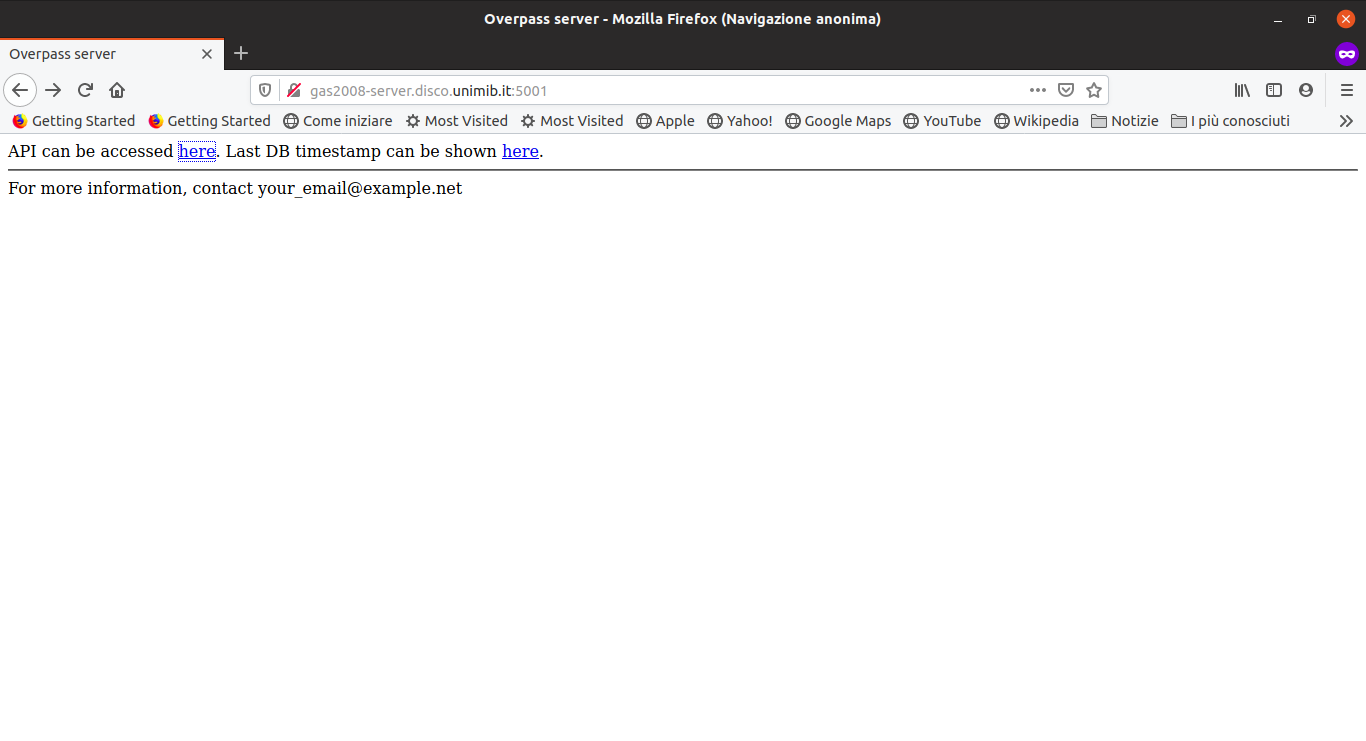
\includegraphics[width=0.7\textwidth]{Immagini/OverpassApiRunning.png}
    \caption{Overpass API in funzione}
    \label{fig:OverpassAPIRunning}
\end{figure}

E' ora possibile sottomettere query all'API utilizzando Overpass QL.
Grazie a Overpass QL possiamo andare ad effettuare query mirate, circoscritte all'interno di bounding box specifiche e andando a chiedere che il risultato contenga delle propietà specifiche
Una query può essere composta da:
\begin{itemize}
    \item Un'istruzione di query che inizia con \textit{"node", "way", "relation", "rel" , "nwr" (node+way+relation)}.
    \item Un' istruzione di output che inizia con \textit{"out"}. 
\end{itemize}

Le query consistono nel tipo di oggetto che dev'essere trovato:
\begin{lstlisting}
node
way
rel
\end{lstlisting}


seguito da almeno una condizione che deve descrivere l' oggetto da trovare ad esempio:\\
\begin{lstlisting}
["name"="Milano"]
\end{lstlisting}

In questo modo è possibile filtrare i singoli tag, cosa necessaria per il nostro progetto.
Infatti è stata costruita la seguente query:

\begin{lstlisting}[caption = {Query di Overpass QL}, captionpos=b,label={lst:OSMQuery}]
[out:json];
(way["building:facade:pcl"]
(37.52871919454917,
    126.91968441009521,
    37.531458875784935,
    126.9231390953064););
(._;>%;);
out meta;
\end{lstlisting}

Ciò consente di restituire tutti le way (e quindi anche i polygon) presenti all'interno del distretto di Yeongdeungpo a Seoul contenenti il tag "building:facade:pcl".

\begin{figure}[H]
    \centering
    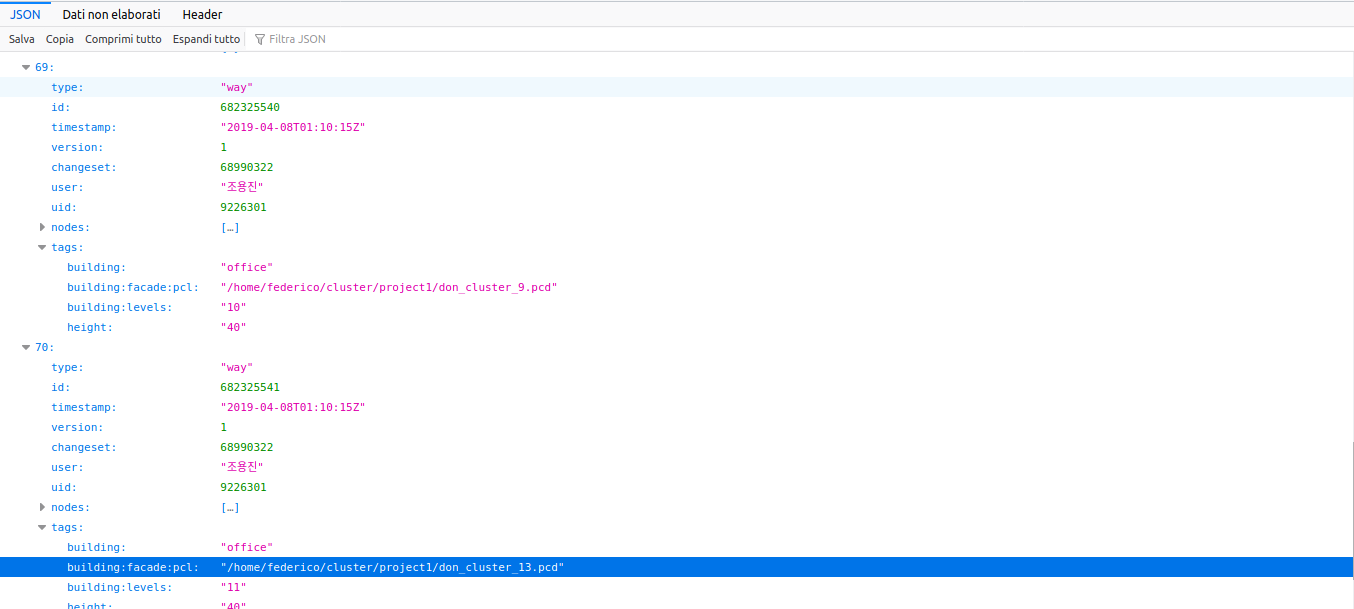
\includegraphics[width=0.7\textwidth]{Immagini/RisultatoQuery.png}
    \caption{Come si può vedere si trovano way con il tag building:facade:pcl presente}
    \label{fig:QueryResult}
\end{figure}

Il risultato della query verrà poi utilizzato per poter recuperare le point cloud quando sarà necessario il loro utilizzo durante il recupero da parte del componente di \hyperref[sez:RLE]{RLE} dedicato.  
\chapter{Recupero e Utilizzo delle Point Cloud}
\label{cap:ReceUsoPCL}

In questo capitolo si descriverà come è stato scritto un servizio di retrival delle pointcloud a partire dalle mappe e di come queste vengano poi utilizzate.

	\section{ROS (Robotic Operating System)}
	\label{sez:ROS}
ROS è un framework flessibile open source che nasce per lo sviluppo e la programmazione dei robot ed è infatti molto utilizzato nell'ambito della robotica di servizio. Il software è liberamente disponibile dal sito ufficiale\cite{ROS}.
Le peculiarità del framework sono simili a quelle di un qualsiasi sistema operativo:
\begin{enumerate}
 \item Capacità di fornire astrazione dell’hardware.
 \item Modularità (cioè la possibilità di avere diverse parti del sistema che lavorano autonomamente al fine di raggiungere un obiettivo comune).
 \item Possibilità di controllare i dispositivi tramite driver. 
 \item Possibilità di gestione delle applicazioni (package).
\end{enumerate}

ROS è costituito fondamentalmente da una rete di processi che vengono eseguiti in parallelo e che comunicano tra di loro sfruttando un architettura Peer-to-Peer.
Essi vengono comunemente chiamati \textit{Nodi} e costituiscono uno degli elementi principali del sistema.
Per essere eseguiti è necessario, innanzitutto, avviare un server principale tramite comando \textit{roscore}. Denominato ROS Master (o Core) consente di effettuare operazioni di routing permettendo ai processi di comunicare tra loro.\\
Nella comunicazione, i \textit{Nodi} si scambiano \textit{messaggi}. ROS fornisce una grande quantità di messaggi predefiniti ma è ovviamente possibile crearne di nuovi a seconda delle proprie esigenze.
Sostanzialmente un nodo è un programma che si interfaccia con il ROS Master per comunicare con altri nodi tramite messaggi.
Il sistema di scambio di messaggi è molto simile all’architettura pub/sub: esistono nodi \textit{talker} (Publisher) e nodi \textit{listener} (Subscriber).\\ 
Per circolare i messaggi possono sfruttare \textit{topic} o \textit{servizi}:
\begin{itemize}
\item \textbf{Topic}: i nodi Publisher creano il Topic (canale di comunicazione) e su di esso pubblicano i messaggi, mentre i nodi Subscriber vi si sottoscrivono per poterne ricevere il contenuto. 
Più nodi possono sottoscriversi allo stesso topic e ogni nodo può pubblicare su uno o più topic contemporaneamente.
\begin{figure}[h!]
    \centering
    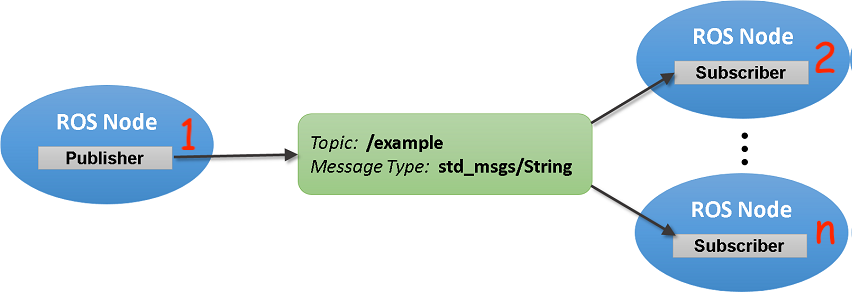
\includegraphics[scale=0.25]{Immagini/topic.png}
    \caption{schema di comunicazione \textit{Publisher-Subscriber} tramite topic}  
    \label{fig:topic}
\end{figure}

\item \textbf{Servizi}: forniscono la possibilità di creare una comunicazione sincrona tra un nodo client, che può richiedere un servizio mandando una \textit{request} ed un nodo server, che riceverà la richiesta e risponderà con una \textit{response}. 
\begin{figure}[h!]
    \centering
    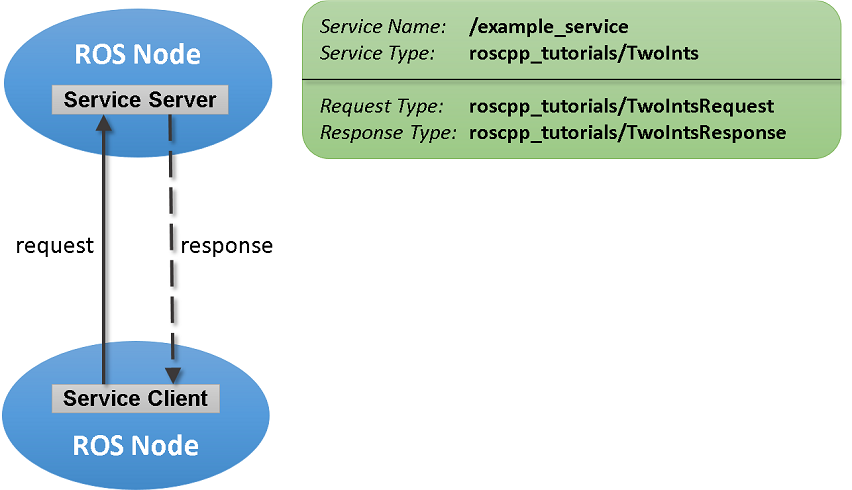
\includegraphics[scale=0.25]{Immagini/servizi.png}
    \caption{schema di comunicazione \textit{Client-Server} tramite servizio}  
    \label{fig:service}
\end{figure}
\end{itemize}

ROS in particolare nella versione Kinetic basata sulla versione 16.04 di ubuntu è alla base di RLE su cui si è andato a lavorare.

\section{RLE (Road Layout Estimation)}
\label{sez:RLE}

\textit{Road Layout Estimation}\cite{Ballardini2015} è un framework probabilistico per l'interpretazione di scene in contesto urbano. Gli elementi da interpretare in una scena urbana possono essere sia di natura \textit{statica}, come edifici, cartelli stradali o incroci, sia di natura \textit{dinamica}, come altri veicoli o persone.

Il framework è modulare e consente la localizzazione attraverso diverse fonti di date. I dati possono provenire da sensori fisici come camere, LiDAR e GPS, o da sensori virtuali ovvero moduli software che analizzano la scena e ne estraggono diverse caratteristiche.

A differenza dei framework già esistenti che prevedono un insieme finito di sensori definito a priori durante la fase di design, \textit{RLE} si basa sull'assunzione che diverse informazioni da diverse fonti possono essere disponibili a frequenze diverse, assenti per un certo periodo, o addirittura utili solo in specifiche situazioni. 

\subsection{Architettura}

L'approccio con cui \textit{RLE} localizza il veicolo nella mappa si basa su un filtro definito particle filtering\cite{thrun2005probabilistic}, la scena viene destcritta attraverso delle \textit{layout hypothesis}(LH). Le LH sono un insieme di elementi che descrivono lo stato del veicolo. In particolare danno informazioni riguardo:

\begin{itemize}

\item Lo \textit{stato} vero e proprio del veicolo, espresso tramite pose e velocità in \textit{6DoF}.

\item Il vettore di \textit{Layout Component}, o LC, ovvero i modelli geometrici o semantici associati agli elementi della scena.

\item lo \textit{score} del layout, ovvero una stima della verosimiglianza dell'ipotesi

\item Il \textit{modello di movimento}, che descrive come l'ipotesi evolve nel tempo.

\end{itemize}

I \textit{layout component}(LC) sono alla base del processo di interpretazione della scena, ogni istanza di LC vive indipendentemente dalle altre, sia che appartengano alla stessa ipotesi o meno, per questo nell'implementazione di ognuna sono definite le funzioni che calcolano sia lo score che la propagazione del moto.

Ogni LC viene creato nel momento in cui \`e riconosciuto da uno specifico detector, che comunica poi al \textit{Layout Manager} i dati di interesse. Il \textit{Layout Manager} \`e il nodo principale del sistema, e il suo compito \`e quello di gestire tutte le diverse ipotesi di struttura della scena nel tempo. Per fare questo assegna a ciascuna ipotesi un punteggio su quanto essa risulti essere verosimile. Di seguito è possibile vedere lo schema ad alto livello di funzionamento del framework.

\begin{figure}[h!]
    \centering
    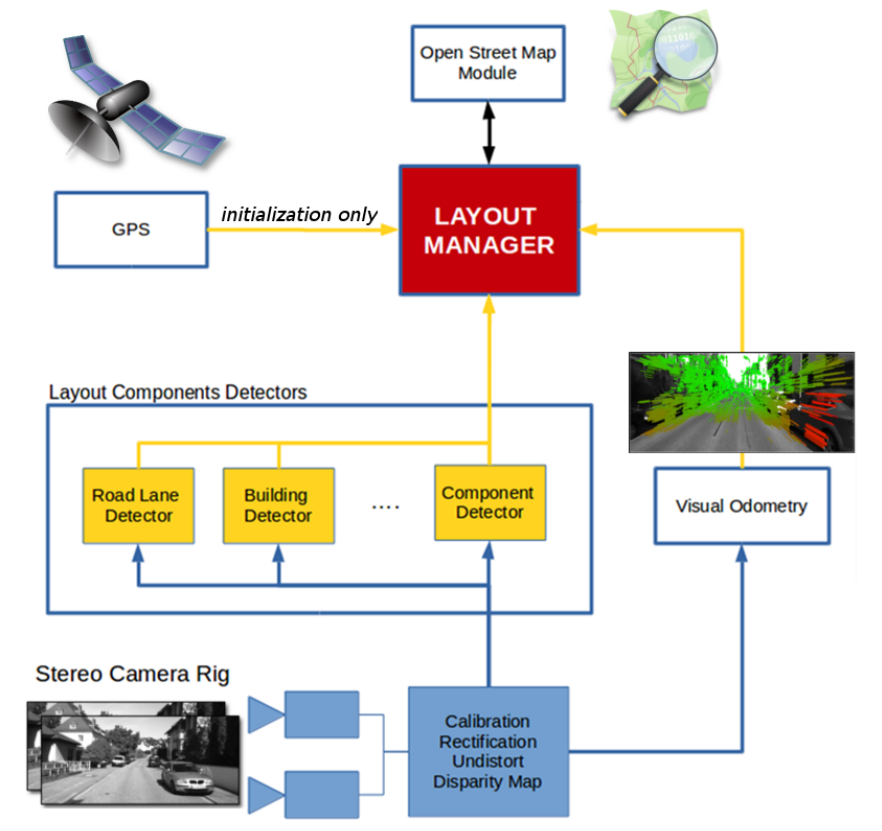
\includegraphics[width=0.8\textwidth]{Immagini/rle.png}
    \caption{Schema ad alto livello del funzionamendo di RLE}
    \label{fig:rle}
\end{figure}

Nel lavoro ci si è concentrati sull'estensione di IRA OpenStreetMaps e di IRA Building Detector\cite{CattaneoSergioTesi} per permettere il recupero e l' utilizzo delle point cloud salvate all'interno delle mappe.

\section{IRA OpenStreetMap}
\label{sez:IRAOSM}
IRA OpenStreetMap è un componente di RLE che consente di caricare le mappe per poi utilizzarle successivamente durante la navigazione, esso è un fork di \href{https://github.com/ros-geographic-info/open_street_map}{ROS Open\_steet\_map} con alcune sostanziali modifiche per il suo utilizzo all'interno di RLE.

Esso è stato modificato in un suo nodo che si occupa dell' acquisizione della mappa. Ad esso sono state fatte delle modifiche riguardanti:
\begin{enumerate}
    \item La selezione della sorgente da cui scaricare la mappa.
    \item La possibilità di scaricare solo gli edifici con una point cloud associata.
\end{enumerate}{}

Per quanto riguarda la prima parte il nodo preesistente consentiva il download soltanto dall'API Overpass globale è stato per tanto necessario inserire la possibilità di utilizzare l'API locale che è stata descritta nel capitolo precedente.\\
Si è quindi aggiunto un argomento booleano \textit{local} al nodo che consente di selezionare su quale server andare ad effettuare la query:

\begin{lstlisting}[caption={Aggiunta del parametro per il download dal server in locale},captionpos=b,language=cpp]
#Aggiunta di un nuovo parametro booleano
TCLAP::SwitchArg localArg("l","local","use local server", cmd, false);
bool local = localArg.getValue();
\end{lstlisting}

Si è poi andato ad introdurre un selettore per selezionare l'url da utilizzare.

\begin{lstlisting}[caption={Selezione del server da utilizzare per la query},captionpos=b,language=cpp]
 if (local){
            osm_api_url = "http://gas2008-server.disco.unimib.it:5001/api/interpreter?data=(" + highwaysQuery + buildingQuery + paramQuery + ");(._;>;);out%20meta;";
        } else {
            osm_api_url = "http://www.overpass-api.de/api/interpreter?data=(" + highwaysQuery + buildingQuery + paramQuery + ");(._;>;);out%20meta;";
        }
\end{lstlisting}

Il secondo punto invece implicava l'inserimento di un nuovo parametro per la scelta di scaricare tutti gli edifici o solamente gli edifici che avevano una point cloud associata. Esso è risultato nell'implementazione all'interno del nodo della query di Overpass API descritta precedentemente \ref{lst:OSMQuery}, aggiunta in modo molto semplice, dopo aver definito il nuovo parametro booleano \textit{buildingPCL} in modo analogo a sopra, con il seguente frammento di codice:

\begin{lstlisting}[caption={Inserimento della query con cui scaricare gli edifici con la PCL associata.},captionpos=b,language=cpp]
if (buildingPCL)
        {
            buildingQuery = "node[building:facade:pcl]" + area + ";"
            + "way[building:facade:pcl]" + area + ";"
            + "relation[building:facade:pcl]" + area + ";";
        }
\end{lstlisting}

E' stato poi necessario implementare un \textit{service} ROS che andasse a recuperare le point cloud ottenute dagli edifici, esso si comporta in modo similare al \textit{service getNearBuildings} già esistente dentro IRA OpenStreetMap  che invece di restituire un messaggio di tipo 
\textit{geometry\_msgs/Point} ovvero una lista di punti restituisse un messaggio di tipo \textit{sensor\_msgs/PointCloud2} ovvero la point cloud che descrive la facciata richiesta in quel momento.\\

Il servizio, denominato \textit{getNearestBuildingFacade}, è definito come segue:

\begin{lstlisting}[caption={Definizione del servizio per il retrival delle facciate},captionpos=b,language=cpp]
#request fields (float64 = C++ double)
float64 latitude
float64 longitude
float64 theta
float64 radius
---
#response fields (float64 = C++ double)
sensor_msgs/PointCloud2 facadecloud
\end{lstlisting}

Il servizio prende in output latitutine, longitudine correnti e i raggi a cui ricercare gli edifici e ritorna la point cloud dell'edificio più vicino, il funzionamento è il seguente:

\subsection{Recupero delle way}
\begin{lstlisting}[caption={Recupero delle way con il tag inerente alla facciata.},captionpos=b,language=cpp]
 Xy center = latlon2xy_helper(req.latitude, req.longitude);
    vector<shared_ptr<Osmium::OSM::Way const> > way_vector;
    for(std::set<shared_ptr<Osmium::OSM::Way const> >::iterator way_itr = oh.m_ways.begin(); way_itr != oh.m_ways.end(); way_itr++
    {
        const char* building_tag = (*way_itr)->tags().get_value_by_key("building:facade:pcl");
        if (!building_tag)
            continue;
        Osmium::OSM::WayNodeList waylist = (*way_itr)->nodes();
        for(Osmium::OSM::WayNodeList::iterator node_list_itr = waylist.begin(); node_list_itr != waylist.end(); node_list_itr++ )
        {
            double lat = node_list_itr->position().lat();
            double lon = node_list_itr->position().lon();
            Xy way_node_xy = latlon2xy_helper(lat, lon);
            double distance = get_distance_helper(center.x, center.y, way_node_xy.x, way_node_xy.y);
            if(distance <= req.radius)
            {
                way_vector.push_back(*way_itr);
                break;
            }
       }
    }
    if(way_vector.size() == 0){
        ROS_ERROR_STREAM("     No map nodes found next to particle. Distance radius: " << req.radius << " m");
        return false;
    }
\end{lstlisting}{}

Questa prima parte è molto similare al servizio già esistente, essa consente di andare a trovare e salvare tutte le way in un raggio ben definito rispetto alla posizione corrente, la differenza rispetto al servizio per il recupero dei generici edifici è che si va a filtrare non solo sul tag \textit{building} che indica se la way è un edificio o meno ma si utilizza il più specifico tag \textit{building:facades:pcl} che indica se un edificio ha una point cloud associata o meno.
\newpage
\subsection{Recupero delle point cloud}
\begin{lstlisting}[caption = {Recupero e download delle pointcloud},numbers=left,captionpos=b, language = cpp]
 for(vector<shared_ptr<Osmium::OSM::Way const> >::iterator way_itr = way_vector.begin(); way_itr != way_vector.end(); way_itr++)
    {
        Osmium::OSM::WayNodeList way_n_list = (*way_itr)->nodes();
        for(Osmium::OSM::WayNodeList::iterator node_list_itr = way_n_list.begin(); node_list_itr != way_n_list.end() - 1; node_list_itr++ )
        {
        const char* facadepclurl = obj.tags().get_value_by_key("building:facade:pcl");
        if (facadepclurl) {
            resource_retriever::Retriever r;
            resource_retriever::MemoryResource resource;
                try
                {    
                    resource = r.get(facadepclurl); 
                }
                catch (resource_retriever::Exception& e)
                {
                    ROS_ERROR("Failed to retrieve file: %s", e.what());
                }
                FILE* f = fopen("cloud.pcd", "w");
                fwrite(resource.data.get(), resource.size, 1, f);
                fclose(f);
                
                sensor_msgs::PointCloud2 output;
                pcl::PointCloud<pcl::PointXYZ> cloud;
                pcl::io::loadPCDFile ("cloud.pcd", cloud);
                pcl::toROSMsg(cloud, output);
                resp.facadecloud = output;
            }
        }
    }
\end{lstlisting}{}

La seconda parte, che si occupa del recupero delle singole facciate rispetto alle way trovate nella parte precedente, può essere suddivisa ulteriormente in 2 parti:
\begin{enumerate}
    \item La parte dalla riga 7 alla riga 20 si occupa del download della point cloud dall'url a cui punta il valore del tag \textit{buildings:facades:pcl}
    \item La parte dalla riga 20 fino alla fine si occupa invece della pubblicazione della PC come messaggio ROS
\end{enumerate}

Il servizio viene poi messo a disposizione per poter essere chiamato dal modulo di building detection\cite{7795618} che effettuerà un confronto tra la point cloud che riceve come messaggi dai vari sensori disponibili (LiDAR o Camere) e la point cloud di riferimento all'interno delle mappe. \\
All'interno di ROS è possibile visualizzare la struttura del servizio che è la seguente:
\begin{figure}[H]
    \centering
    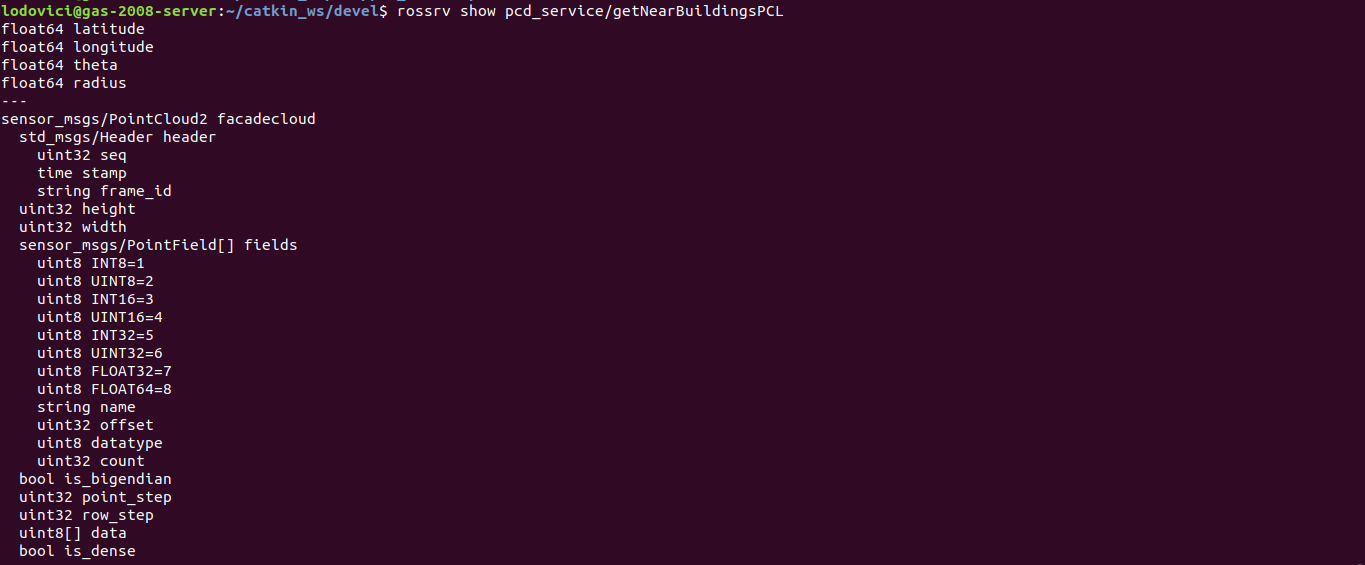
\includegraphics[width=0.9\textwidth]{Immagini/strutturamessaggio.png}
    \caption{Struttura del servizio di richiesta delle point cloud}
    \label{fig:QueryResult}
\end{figure}

Il servizio è stato poi testato facendo delle richieste grazie a \textit{rosservice call} che permette di interrogare i servizi ros
\begin{figure}[H]
    \centering
    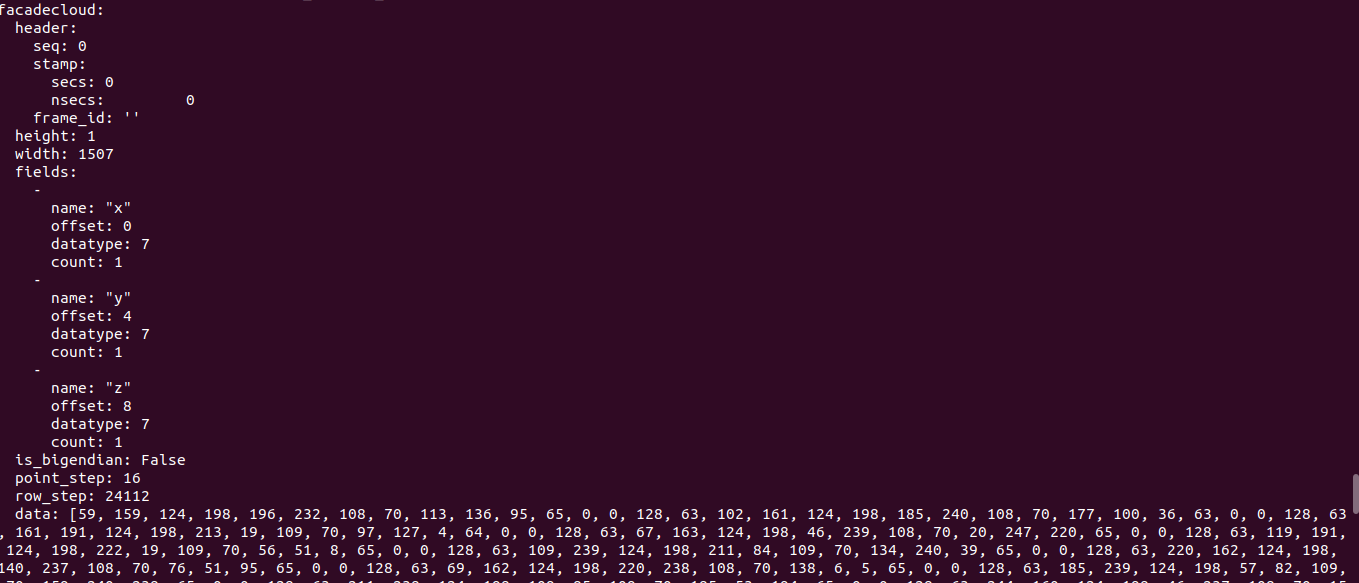
\includegraphics[width=0.9\textwidth]{Immagini/RispostaAlServizio.png}
    \caption{Si può notare che il servizio risponde con una pointcloud contenente la facciata dell'edificio corrente}
    \label{fig:QueryResult}
\end{figure}
\chapter{Conclusioni}
\label{cap:Conclusioni}
L'obiettivo del lavoro è stato quello di ottenere una pipeline funzionante che potesse mettere a disposizione, incorporandole nelle mappe, informazioni aggiuntive riguardanti le facciate degli edifici attraverso le point cloud che le descrivono.\\
Il sistema è risultato funzionante e facilmente riproducibile, il lavoro potrà quindi essere utilizzato per testare se esiste un miglioramento sostanziale dell'accuratezza di localizzazione attraverso l'utilizzo di mappe aumentate. Durante la prototipazione della pipeline sono stati fatti alcuni passaggi manuali che possono essere facilmente automatizzati con l'ausilio di script dedicati che potranno essere svilupppati in seguito, in particolare l'aggiunta del tag che rappresenta le facciate all'interno di OSM è facilmente automatizzabile attraverso l'utilizzo di librerie dedicate.\\
La parte di segmentazione ha dato risultati ottimali solo su specifici dataset con poche fonti di disturbo come alberi e segnali stradali, per tanto è necessario trovare e utilizzare un modello per la segmentazione delle facciate più robusto, in grado di funzionare in una maggior quantità di scene. 
Inoltre si potrebbero sottomettere le modifiche effettuate alle mappe "globali" in modo da eliminare la necessità di utilizzarne una loro istanza locale, ciò ha tuttavia problemi legislativi ed è, al momento, impossibile.

\newpage
\addcontentsline{toc}{chapter}{Lista delle Immagini}
\listoffigures\newpage
\addcontentsline{toc}{chapter}{Lista del Codice}
\lstlistoflistings\newpage
\nocite{*}
\printbibheading[heading=bibintoc, title={Riferimenti}]
\printbibliography[nottype=online,heading=subbibintoc,title={Bibliografia}]
\printbibliography[type=online,heading=subbibintoc,title={Siti}]

\end{document}